\documentclass[journal]{IEEEtran}

\usepackage[pdftex]{graphicx}
\usepackage{amsmath}
\usepackage{algorithmic}
\usepackage{cleveref}
\usepackage{url}

\begin{document}

\title{In-situ visualization of natural hazards with Galaxy and Material Point Method}
\author{Greg Abram, %~\IEEEmembership{Fellow,~OSA,}
        Andrew Solis,
        Yong Liang,
        and~Krishna Kumar% <-this % stops a space
\thanks{Department of Civil, Architectural and Environmental Engineering, University of Texas at Austin, TX, 78712 USA e-mail: (krishnak@utexas.edu).}% <-this % stops a space
\thanks{Texas Advanced Computing Center, University of Texas at Austin, TX,.}% <-this % stops a space
\thanks{University of California at Berkeley, CA,.}% <-this % stops a space
\thanks{Manuscript received September 3rd, 2021.}}

% The paper headers
\markboth{IEEE Computing in Science and Engineering (CiSE), Special Issue 2021}%
{}

%\IEEEpubid{0000--0000/00\$00.00~\copyright~2015 IEEE}
% use for special paper notices
%\IEEEspecialpapernotice{(Invited Paper)}

% make the title area
\maketitle

% As a general rule, do not put math, special symbols or citations
% in the abstract or keywords.
\begin{abstract}
Visualizing regional-scale landslides is the key to conveying the threat of natural hazards to stakeholders and policymakers. Traditional visualization techniques are restricted to post-processing a limited subset of simulation data and are not scalable to rendering exascale models with billions of particles. In-situ visualization is a technique of rendering simulation data in real-time, i.e., rendering visuals in tandem while the simulation is running. In this study, we develop a scalable N:M interface architecture to visualize regional-scale landslides. We demonstrate the scalability of the architecture by simulating the long runout of the 2014 Oso landslide using the Material Point Method coupled with the Galaxy ray tracing engine rendering 4.2 million material points as spheres. In-situ visualization has an amortized runtime increase of 2\% compared to non-visualized simulations. The developed approach can achieve in-situ visualization of regional-scale landslides with billions of particles with minimal impact on the simulation process.
\end{abstract}

% Note that keywords are not normally used for peerreview papers.
\begin{IEEEkeywords}
In-situ visualization, Material Point Method, TACC Galaxy, Ray tracing.
\end{IEEEkeywords}

\IEEEpeerreviewmaketitle

\section{Overview and motivation}
% - why simulating earthquakes is important
% - why such sim is hard
% - brief description of MPM and benefits, cite to marker paper
% - why in situ vis is needed / benefits
% - Galaxy + MPM = awesomeness
\IEEEPARstart{L}{andslide} runouts are regional-scale events that can bury whole towns (e.g., 2018 Southern California mudflows that followed a series of wildfires, 2014 Oso landslide caused 43 fatalities in the US) or devastate entire regions (e.g., 2016 Kaikoura, New Zealand earthquake recorded 100,000 landslides within a 12,000 sq. km area). The frequency of these regional-scale landslides is increasing with devastating earthquakes, extreme precipitation, and wildfires caused by climate change. Even in these risk-prone communities, where the residents are aware of the threat posed by the landslides, the residents repeatedly show indifference to these threats and consequently fail to act. The human capacity to deny danger endangers lives and property~\cite{kim2020public}. In 2020, twenty-two extreme events cost the United States \$95 billion in damages. The underlying problem is the uncertainty of the actual event and a lack of understanding of its potential impacts. How to communicate the reality of potential risk to a diverse group of individuals, who must understand and support a complex set of actions that reduce the risk for the whole community?
  
Visualization is the key to communicating scientific results effectively to engineering decision-makers and the public. Given the limited cognitive capacity in humans, visualizing the complex threats as images enhances the brain's capacity to perceive opportunities and make decisions. Visual representation of complex information reduces the cognitive load on human information processing and increases human ``absorptive capacity" for problem-solving~\cite{kahneman2012human}. However, these visualizations must be physically sound to be perceived as realistic and accepted as valid. Visualization is also context and user-specific, i.e., different users may be interested in different aspects of the experimental or simulation data sets. Hence, the same data set may be represented in several forms – perhaps at varying levels of detail, emphasizing or deemphasizing different regions and features, and employing different visualization techniques to best present the information.

Despite the landslide risks, most regional-scale landslide hazard analyses do not consider downstream impacts and the aerial extent of debris-flow runouts~\cite{USGS2017debris}. Traditional numerical methods such as the Finite Element Method (FEM) primarily focuses on the onset of failure but provides limited information on the post-failure runout mechanisms due to mesh distortions at large  deformations~\cite{soga2016trends}. Modeling the impacts of the potential runout of large landslides is possible with new tools such as Material Point Method (MPM)~\cite{kumar2019scalable}. MPM is a mesh-free method that discretizes the domain as a collection of \textit{material points} moving on a background grid, and Newton's laws of motion determine their deformations. In this study, we employ the CB-Geo MPM code (\url{https://github.com/cb-geo/mpm}), and a typical MPM computation cycle is shown in~\cref{fig:mpm}. For more information on MPM and the code implementation, refer to~\cite{kumar2019scalable}. MPM results of the landslide runout can be translated into compelling visualizations to inform decision-makers of potential hazards. 


\begin{figure}[!htbp]
    \centering
    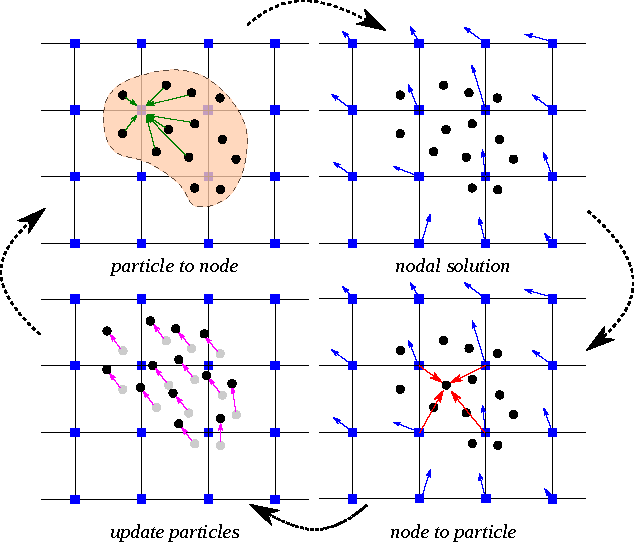
\includegraphics[width=\linewidth]{figs/mpm.pdf}
    \caption{Illustration of the MPM algorithm (1) A representation of material points overlaid on a computational grid. Arrows represent material point state vectors (e.g., mass, volume, and velocity) is projected to the nodes of the computational grid. (2) The equations of motion are solved onto the nodes, resulting in updated nodal velocities and positions. (3) The updated nodal kinematics is interpolated back to the material points. (4) The state of the material points is updated, and the computational grid is reset.}
    \label{fig:mpm}
\end{figure}

A regional-scale landslide simulation of a kilometer-scale runout with MPM requires billions of material points and millions of cells in the background grid. Scaling applications to simulate a billion particles require exascale high-performance computing (HPC) architectures with efficient Message-Passing Interface (MPI). This study uses the CB-Geo MPM code, which exploits a hybrid MPI+X approach to achieve regional-scale simulation of landslides. In addition, as the landslide runout progresses, the workload distributed across the compute nodes becomes imbalanced. We adopt a distributed graph-partitioning technique to load balance both the background mesh and particle distribution dynamically.

Data retrieval and visualization in High-Performance Computing applications have long been a bottleneck. Current techniques for visualizing exascale simulations involve writing a temporal slice of a subset of the data to disk, often at a much coarser resolution than the original data, which leads to a significant portion of information being disregarded and potentially lost, followed by post-processing. In practice, this usually means that the data are stored only at specific time steps. An exascale simulation would output terabytes of data, resulting in a significant portion of the compute time spent on I/O~\cite{byna2020exahdf5}. Nevertheless, the scale of such discrete geometry visualization will push commercial rendering engines like Mantra and Arnold to the limit. The amount of data would be several orders of magnitude higher at exascale levels, making the simulation spend most of the compute time in I/O.

Running the visualization and simulation in tandem avoids data transfer bottleneck, enabling scientists to monitor and modify simulation parameters in real-time. In-situ visualization libraries such as ParaView Catalyst and SENSEI offer the ability to couple existing data models (such as VTK) to query regions of interest and to render simulations. However, scaling rendering engines to exascale simulations remains a challenge requiring billions of lightpaths to be rendered. Most rendering engines only sample a limited number of random light paths at each step. Thus, the visual quality of rendered images suffers from estimator variance, which appears as visually distracting noise~\cite{yang2021foveated}. Ray tracing engines such as TACC Galaxy~\cite{abram2018galaxy} (\url{https://github.com/cb-geo/mpm}) offer distributed asynchronous in-situ visualization capabilities for exascale simulations. 

This study develops an in-situ visualization technique to simulate and render regional-scale landslides by coupling the CB-Geo MPM code for large-deformation modeling with distributed asynchronous ray tracing engine TACC Galaxy. In this study, we apply the in-situ visualization technique in MPM to simulate and visualize the disastrous 2014 Oso landslide, also known as the SR 530 landslide, which occurred in the northwest Washington state in the US, resulting in an 1100 m runout. 

\begin{figure}[!htbp]
    \centering
    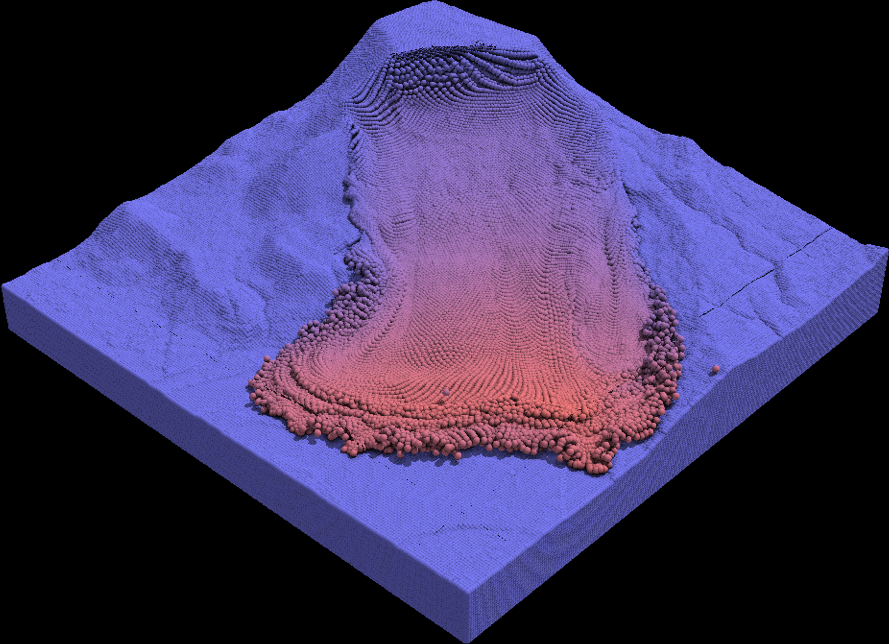
\includegraphics[width=\linewidth]{figs/osofull.png}
    \caption{Visualization of a timestep of the MPM simulation of the Oso landslide.   Particles are represented as spheres with a radius approximating the original resolution.  Color represents the distance of each particle from its original location.} 
    \label{fig:osofull}
\end{figure}

\Cref{fig:osofull} shows a visualization of the final runout of the MPM simulation of the Oso landslide.   In this case, we use Galaxy to render the scene using spheres to represent the material points in the simulation, each with a fixed radius matching the original particle grid resolution and colored by the distance between each particle's current and original location.  Galaxy's global lighting model is used to calculate shadows for additional depth perception.

\section{Related work}
\subsection{Visualization Systems}
Systems for visualizing large-scale scientific data have been available for decades. High-performance graphics engines - add-ons to powerful workstations first made interactive post-processing visualization of large datasets possible in the 1980s, leading to visualization systems like AVS, IBM Data Explorer, and Silicon Graphics IrisExplorer. These systems and others forged a visualization paradigm in which non-sophisticated users, i.e., non-programmers, could use graphical user interfaces to develop specific visualizations of their data and provide real-time interactive data exploration.  

In the early days, such high-performance visualization engines were expensive and capable only of low-level rendering functions and were limited to dedicated visualization systems.  This separation of simulation and visualization led to a distinction between general-purpose computation systems for running simulations and graphics-capable systems for visualization.  Based on a \textit{post-processing} workflow paradigm, simulations would run first on general-purpose systems, then transferred to separate systems for visualization.  Post-processing remains the standard approach to visualizing large-scale data.

Today, simulation have outstripped the capabilities of even the most heavyweight conventional processors, leading to the development of today's supercomputers - \textit{clusters} of conventional processors (referred to as \textit{nodes}) with very high-speed intercommunications, requiring simulation applications (such as MPM) incorporate sophisticated algorithms to distribute the workload over many cooperating nodes. To keep up, visualization systems have also adopted a distributed-parallel architecture; popular general-purpose systems (notably Paraview and VisIt) have been adapted to distributed-memory parallel systems to provide visualization capabilities for simulation systems to run on the largest systems in the world.

\subsection{In-situ Visualization}

Unfortunately, the I/O capabilities of such systems have not matched their computational capabilities, making it even more expensive to export data from the simulation system memory to secondary storage and subsequently read it back into visualization system memory.  This leads to a tension between the expense of saving time-step data and the requirements of visualization.
  
\textit{In-situ} visualization is a broad approach to processing simulation data in real-time - that is, \textit{wall-clock} time, as the simulation is running.  Generally, the approach is to provide \textit{data extracts}, which are condensed representations of the data chosen for the explicit purpose of visualization and computed without writing data to external storage.  Since these extracts (often images) are vastly smaller than the raw simulation itself, it becomes possible to save them at a far higher temporal frequency than is practical for the raw data, resulting in substantial gains in both efficiency and accuracy.  In-situ visualization allows simulations to export complete datasets only at the temporal frequency necessary for economic checkpoint/restart. 
 
Many approaches to in-situ visualization exist.  In \cite{Childs:IJHPCA}, Childs et al. provide an exhaustive taxonomy of approaches, differentiating along six axes: the type of integration between simulation and visualization components;  how the components are situated on computing resources, how the visualization components access simulation data, timing, control, and output type.  For a complete discussion, please refer to the paper.  The paper also offers a survey of existing in-situ systems.  Both Paraview and VisIt provide in-situ capabilities; each provides an interface (Catalyst and libsim) with which data is transferred from the simulation code to co-resident visualization components; the simulation code then transfers control to the visualization components, resuming only when the visualization components return.
 
\subsection{Rendering Techniques}
At run-time, visualization consists of two phases: converting raw data to renderable primitives (generally triangles) and transferring data to a rendering subsystem that produces pixels in an image buffer.  Traditionally, this rendering process uses the \textit{rasterization} and Z-buffer algorithms to generate pixels. This approach, implemented in hardware, considers each primitive independently, determining which pixels are affected by the primitive, and for each such pixel, it evaluates how far it is from the viewpoint. If a given is the closest so far (by comparing depth with the current value in the Z-buffer), it is shaded, saved to the image buffer, and its depth to the Z-buffer.  Since this algorithm touches all the primitives, the cost is O(n), where n is the number of primitives.

More recently, this approach is being replaced by \textit{ray-tracing}.  In this algorithm, the rendering loop is across all pixels in the image, asking which primitive is visible at the pixel.  This algorithm relies on an O(log n) search for each pixel and, on today's hardware (both general-purpose multi-core vector CPUs and graphics cards), is competitive in speed with rasterization and provides additional capabilities.  First, ray tracing provides a simple approach to realistic lighting effects - notably shadowing - that are hard to implement in rasterization algorithms.  Both VisIt and Paraview optionally replace their traditional scan-conversion rendering with ray tracing, utilizing Intel's CPU-based OSPRay and Nvidia's GPU-based Optix.  

The second advantage of the ray tracing algorithm is that, in some critical cases, it avoids the necessity of reducing data to low-level geometric primitives.  Critical to the current work is that the rendering of spheres in a rasterization algorithm requires that each sphere be represented as a set of triangles sufficiently large enough to give the appearance of a smooth sphere.   When there is a large number of spheres to render, rasterization (which recall considers every triangle) becomes very expensive.  Instead, using ray tracing, we can represent each sphere by its center and radius; rather than exhaustively intersect a ray against each triangle of a sphere's tessellated representation, we can determine the distance between the ray and the center and ask whether it is less than the radius.  This feature is apparent in Paraview; while the traditional rasterization back end required a filter to create spheres of each point, the points can be rendered directly using the OSPRay back end with substantially improved performance.

\subsection{Parallel Rendering}
When visualizing on multiple nodes in parallel, the resulting image may contain imagery computed on any participating node. To get a correct image, visualization systems generally use one of two algorithms. First, they can redistribute the primitives to provide all the information necessary to render a screen patch (possibly the entire image).  Alternatively, each node renders its portion of the data independently and then uses a distributed-parallel depth-based compositing algorithm to reconcile these partial results into a final image. Each has advantages: if the amount of data required to render the image is small, it can be gathered cheaply and then rendered interactively with no further data movement.  On the other hand, when the data is large, the gather is expensive (and potentially exceeds the memory available on the rendering node(s)), and the post-rendering compositing step is preferable.

When advanced global lighting is required, we note that the second of these algorithms will not work.  Without shadows, the correct shading for a surface is determined independently of other surfaces and thus can be performed locally before compositing.  When shadows are required, the surface can be shadowed by a surface \textit{that is not present on current node}.  Thus post-rendering compositing cannot create a correct image, leaving gathering the data as the alternative.

Galaxy, developed at TACC, differs from OSPRay and Optix in that it is based on a regular partitioning of the computational space, with all the data contained in each partition local to the node responsible for the partition. This assumption - derived from the spatial partitioning commonly used in distributed-memory simulation systems - allows Galaxy to do \textit{most} of the work locally, considering (on average) only 1/N of the data, and transferring rays in a nearest-neighbor pattern only when rays (primary and secondary) exit one partition and enter another.  Rays are retired when they are resolved, and results are transferred to a potentially remote frame buffer.
 
\subsection{Providing Interactive Visualization In-Situ}
Of course, in-situ visualization largely precludes exploratory visualization: the in-situ analysis will only produce the anticipated results at set-up time.  With post-processing, the entire dataset is available when the user sits down in front of the visualization system; the user can adjust viewpoints and parameters interactively during his session, a powerful capability lost in in-situ visualization. However, Ahrens et al. \cite{Ahrens2014cinema} observed that, for the cost of writing a single timestep of the simulation data, we could save many \textit{images} of the timestep.  Therefore, we can set up an in-situ process that generates as many images of the data - varying viewpoints and parameters - as the user anticipates and wants. Ahrens et al. have developed a database format storing these images, and Cinema - a browser for the interactive exploration of such databases.  We can, for example, specify a range of viewpoints in angle and distance and generate an image for each timestep; the Cinema browser will then present an interactive window giving the appearance of being able to interact with the data in 4 dimensions in real-time.

\section{Study Detail}
The 3D Oso landslide region of interest spans 1500 x 1500 x 270 m. This domain is discretized into 4.2 million material points and a background grid of 8 x 8 x 8 m. In most regions, we use two material points in each direction (8 material points per cell), while the sliding area has a higher resolution with four material points in each direction (64 points per cell). A Mohr-Coulomb material model with a Total Stress Approach is used to simulate the undrained runout evolution of the Oso landslide in MPM. 

In this work, we consider in-situ visualization for MPM. In particular, we note that the data for visualization is simple: a large set of points with scalar attributes (currently ~4.2M and potentially billions), scattered among a large number of parallel processes.  The objective is to generate potentially many images at an appropriate temporal frequency and minimize the need for MPM to dump timestep data.  We would like to do so with minimal impact on both the MPM codebase (minimizing additional code and dependencies) and the run-time, minimizing the impact on MPM's run-time memory footprint and performance.  Finally, we would like this interface to be intermittent, allowing us to connect a visualization to a running instance of MPM, enabling us to examine the current state of the simulation.

We chose Galaxy, our ray-tracing-based visualization system, to interface to MPM.  Galaxy has several advantages that make it attractive in this use; using the compact representation of spheres as the center with radius, rendering a significant number of spheres efficiently, and scaling as necessary to provide the desired performance.  Ideally, we would like to balance the performance of the MPM simulation with the Galaxy visualization; by developing an M:N point-to-point interface between MPM worker processes and Galaxy processes, we can vary the number of processes in each so that they run at approximately the same pace.  When out of balance, we can choose to drop frames of the visualization by having MPM continue without pausing if Galaxy is not ready, or not - by having MPM wait for Galaxy to \textit{be} ready.

\subsection{The Interface}

We use a sockets-based interface for this preliminary work, enabling the two components to communicate via the IP protocol.  While this enables us to position the components anywhere with IP connectivity, by placing the two on the sample supercomputer, we are able to use the full parallel bandwidth of the supercomputer's interconnect to communicate between MPM and Galaxy worker processes.

We use a single connection between the root processes of MPM and Galaxy to control the overall process. When Galaxy is launched, its root process creates a master server socket and waits for the simulation's root process to connect. Each worker process opens a server socket and waits for zero or more simulation workers to connect.

Periodically, the MPM root process (at its synchronization point) attempts to connect to this server based on a host/port pair given in its configuration file (we generally leave this as localhost/1900 and use an SSH tunnel to connect that local port to wherever the Galaxy root process is running). A small amount of control information is passed when the connection is established, including a list of host/port pairs for listening Galaxy worker processes and the number of MPM worker processes transferring data. This lets each MPM worker know where to send its data, and each Galaxy worker knows how many connections to expect. Data transfer occurs in parallel, and MPM continues when the transfers are complete.

\subsection{Data}

We have implemented an ad-hoc data structure for passing data from MPM to Galaxy for this preliminary work.  This format consists of a small header containing the name of the variable being transferred and the number of points/data values, followed by a block of binary floats comprising the points, followed by the binary float scalar data values for each point.

\subsection{Galaxy Side}

Once data has arrived on the Galaxy side, it is re-distributed into a Galaxy-compliant partitioning of the computational space.  As mentioned above, Galaxy relies on a regular subdivision of space - which is not the case for data acquired from MPM, particularly in that multiple MPM workers can send data to each Galaxy node.  Since each Galaxy worker knows the overall partitioning, this reshuffle is performed using point-to-point messaging via MPI.  Each worker reads and writes approximately 1/N of the data after examining 1/N of the data.  We note that while this repartitioning accrue cost, this cost is amortized across all visualization time steps~\cite{abram2018galaxy}.

\subsection{Specifying the Visualization}

Galaxy uses a JSON text file (a \textit{state} file) to specify a visualization.  The JSON consists of several sections describing: the data objects, the distinct visualizations, listing the data objects and operators to be applied to the lighting environment, a list of cameras, and renderer parameters.  Names in the data object section correspond to the variables in MPM; at setup time, Galaxy creates empty distributed containers for each named object.  At run time, the results of reshuffling data received from MPM replace the contents (if any) of these distributed data objects.  

From the state file, Galaxy generates a \textit{RenderingSet}, consisting of a list of individual renderings, one for each visualization/camera pair.  Executing the RenderingSet causes the renderings to be initiated simultaneously, and individual image files are generated.

Galaxy has a state-file generator program for Cinema.  A \textit{.cinema} file is similar to that specifies \textit{ranges} of parameters, \textit{cinema2state} generates a single state file that contains a list of the visualizations described in the input file with every combination of parameter settings, and a list of cameras with all the combinations of viewpoint parameters.  Galaxy will generate a complete Cinema database with an interactor for each varying parameter and time.

\section{Results}
\begin{figure}[!tbp]
    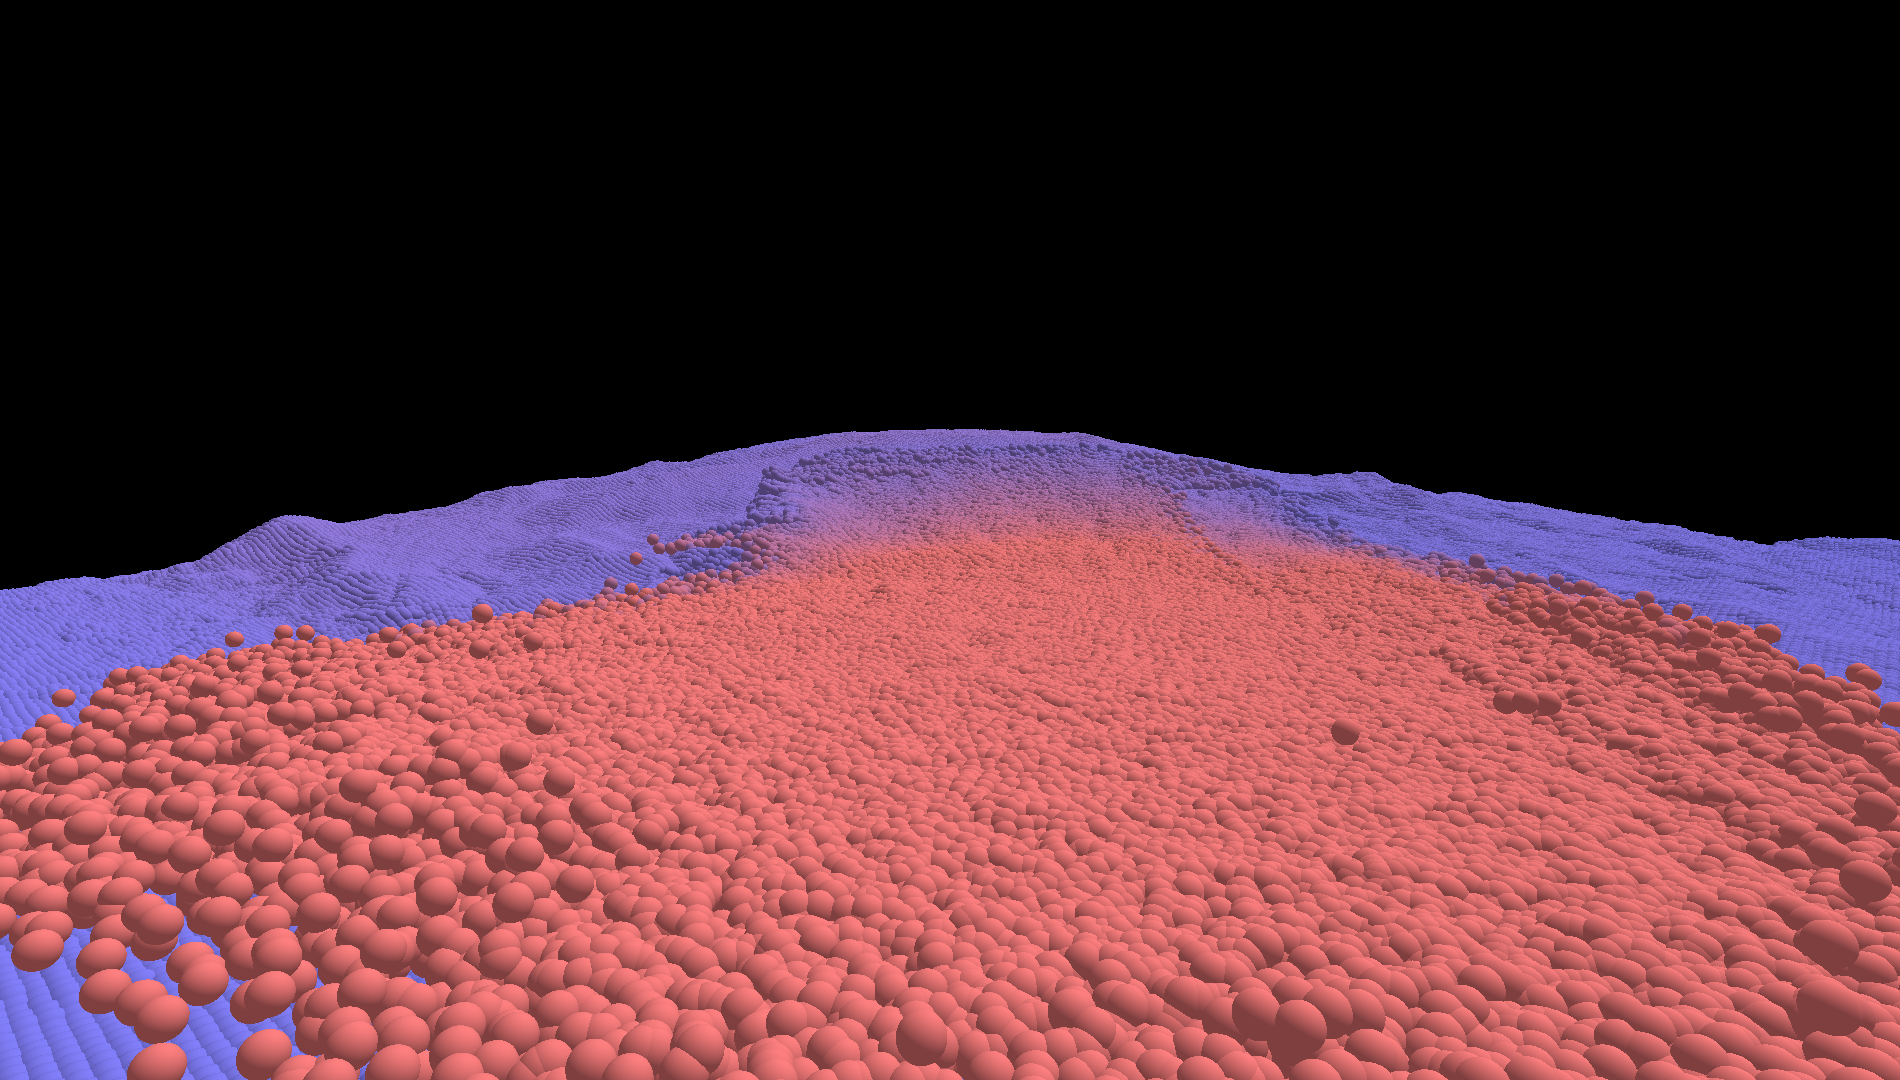
\includegraphics[width=\linewidth]{figs/timestep-0000.png}
    \caption{Oso Landslide early}
    \label{fig:oso-early} 
\end{figure}
\vspace{0.2cm}
\begin{figure}[!tbp]
  \centering
    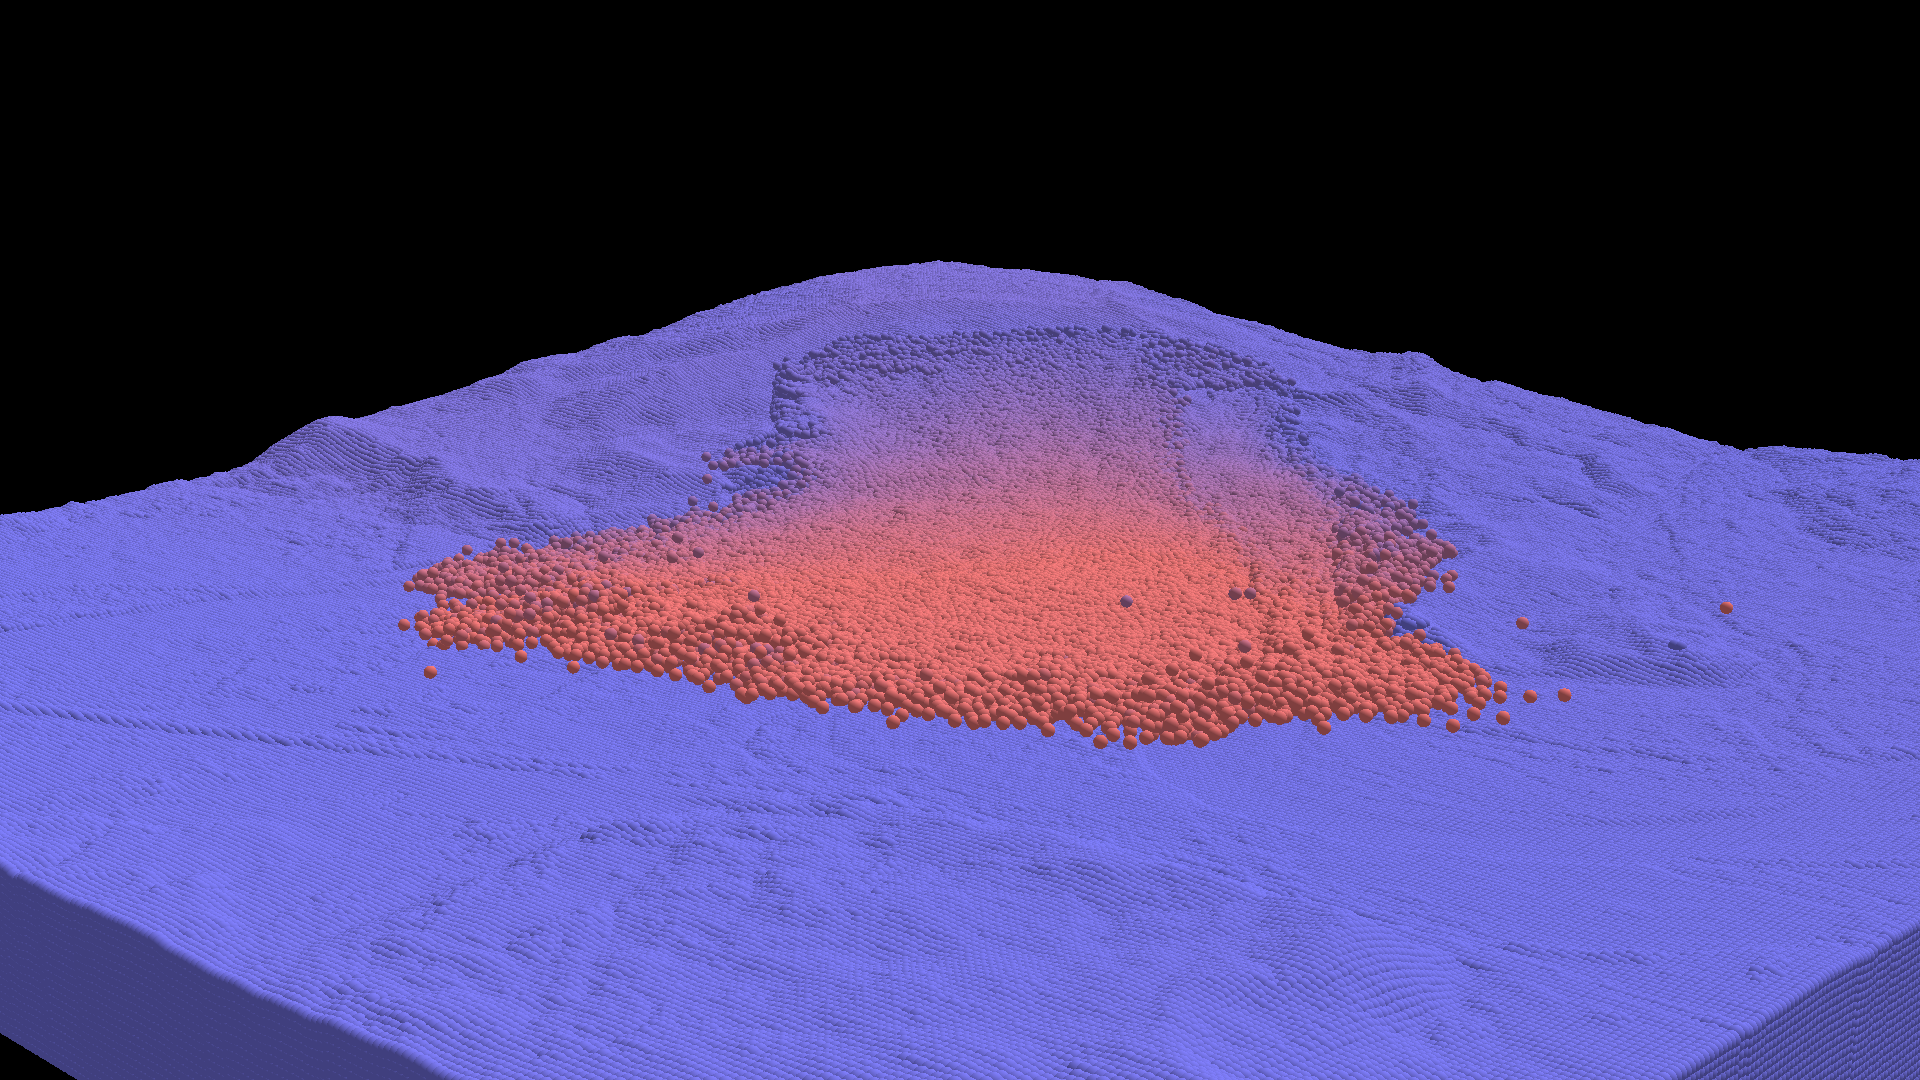
\includegraphics[width=\linewidth]{figs/timestep-0253.png}
    \caption{Oso Landslide late}
    \label{fig:oso-late}
\end{figure}

Given a checkpoint restart file at step 50,000 of the MPM Oso simulation, we ran two versions of the next 15,000 steps to evaluate the cost of in-situ visualization on the simulation.   Using four nodes of Stampede2 at TACC, each running four MPM worker processes, we first ran 15,000 steps without in-situ visualization but saving checkpoint files every 500 steps.  In this case, the wall-clock time required to run each 5,000 steps - as determined by timestamps on output files - was approximately 2 hours, 23 minutes.

We then reran the same section of the simulation using the MPM/Galaxy interface to transfer data from MPM to Galaxy every 100 steps and using Galaxy to generate the first two and later three images of each timestep (having noted the runout spread outside our initial camera views) of each step.  Figures \ref{fig:oso-early} and \ref{fig:oso-late} show two views of this run.

In this case, 
we ran Galaxy using four worker processes on a single node, so there was a 4:1 ratio of both sending processes to receiving process and sending nodes to receiving nodes.   Galaxy required approximately 3 seconds for each timestep to receive the data, repartition it, and render the visualizations - far less than the ~three minutes required by MPM to run through 100 steps.   In this second case, the wall-clock time needed by MPM to run through 5,0000 steps was approximately 2 hours, 26 minutes, or 2 percent more than the first, non-visualized case.

\section{Conclusion}

The above demonstrates that, at this scale, the time cost of in-situ transfer of data from this simulation to a visualization application located on a separate partition of the same supercomputer is negligible.   Further, the time required to generate the three simple views of the data for every 100 timesteps is much less than the cost of simulating 100 timesteps, indicating that more elaborate visualization (for example, generating many views of each timestep, enabling Cinema-based, real-time interaction the visualization) is achievable without impacting the simulation.

We realized that a new view was necessary to capture the full extent of the run-out at mid-run.   We were able to re-parameterize the visualization on the fly to add this additional view.   

\subsection{Future work}

Clearly, the test example we have worked with - the Oso landslide at a relatively coarse resolution does not tax our system.   However, as observed above, regional-scale simulation of landslides resulting in kilometer-scale runout will require billions of particles rather than millions.   We believe our approach - notably using a scalable visualization component (Galaxy, \cite{abram2018galaxy}) and a scalable N:M interface architecture enables us to re-scale the visualization process as necessary to achieve in-situ visualization of simulation data with minimal impact on the simulation process.  

\appendices

% use section* for acknowledgment
\section*{Acknowledgment}
The simulations and in-situ visualization of the Oso landslide were conducted on the Texas Advanced Computing Center’s (TACC’s) cluster Stampede2.  Krishna Kumar would like to thank the U.S. National Science Foundation grant CMMI-2022469. Greg Abram would like to thank the U.S. Department of Energy grant DE-SC0012513. However, any opinions, 
findings and conclusions or recommendations expressed in this material are those of the authors and do not necessarily reflect the views of the National Science Foundation.

% Can use something like this to put references on a page
% by themselves when using endfloat and the captionsoff option.
\ifCLASSOPTIONcaptionsoff
  \newpage
\fi

% trigger a \newpage just before the given reference
% number - used to balance the columns on the last page
% adjust value as needed - may need to be readjusted if
% the document is modified later
%\IEEEtriggeratref{8}
% The "triggered" command can be changed if desired:
%\IEEEtriggercmd{\enlargethispage{-5in}}

% references section

% can use a bibliography generated by BibTeX as a .bbl file
% BibTeX documentation can be easily obtained at:
% http://mirror.ctan.org/biblio/bibtex/contrib/doc/
% The IEEEtran BibTeX style support page is at:
% http://www.michaelshell.org/tex/ieeetran/bibtex/
\bibliographystyle{IEEEtran}
% argument is your BibTeX string definitions and bibliography database(s)
\bibliography{IEEEabrv,references.bib}
%
% <OR> manually copy in the resultant .bbl file
% set second argument of \begin to the number of references
% (used to reserve space for the reference number labels box)
%\bibliography{references.bib}

% biography section
% 
% If you have an EPS/PDF photo (graphicx package needed) extra braces are
% needed around the contents of the optional argument to biography to prevent
% the LaTeX parser from getting confused when it sees the complicated
% \includegraphics command within an optional argument. (You could create
% your own custom macro containing the \includegraphics command to make things
% simpler here.)
%\begin{IEEEbiography}[{\includegraphics[width=1in,height=1.25in,clip,keepaspectratio]{mshell}}]{Michael Shell}
% or if you just want to reserve a space for a photo:

% \begin{IEEEbiography}{Michael Shell}
% Biography text here.
% \end{IEEEbiography}

% if you will not have a photo at all:
% \begin{IEEEbiographynophoto}{John Doe}
% Biography text here.
% \end{IEEEbiographynophoto}

%\vfill

% Can be used to pull up biographies so that the bottom of the last one
% is flush with the other column.
%\enlargethispage{-5in}
\end{document}


